\documentclass{article}

\usepackage{amsmath, amsthm, amssymb, amsfonts}
\usepackage{thmtools}
\usepackage{graphicx}
\usepackage{setspace}
\usepackage{geometry}
\usepackage{float}
\usepackage{hyperref}


\usepackage[utf8]{inputenc}
\usepackage[english]{babel}
\usepackage{framed}
\usepackage[dvipsnames]{xcolor}
\usepackage{tcolorbox}

\colorlet{LightGray}{White!90!Periwinkle}
\colorlet{LightOrange}{Orange!15}
\colorlet{LightGreen}{Green!15}

\newcommand{\HRule}[1]{\rule{\linewidth}{#1}}

\declaretheoremstyle[name=Theorem,]{thmsty}
\declaretheorem[style=thmsty,numberwithin=section]{theorem}
\tcolorboxenvironment{theorem}{colback=LightGray}

\declaretheoremstyle[name=Proposition,]{prosty}
\declaretheorem[style=prosty,numberlike=theorem]{proposition}
\tcolorboxenvironment{proposition}{colback=LightOrange}

\declaretheoremstyle[name=Principle,]{prcpsty}
\declaretheorem[style=prcpsty,numberlike=theorem]{principle}
\tcolorboxenvironment{principle}{colback=LightGreen}

\setstretch{1.2}
\geometry{
    textheight=9in,
    textwidth=5.5in,
    top=1in,
    headheight=12pt,
    headsep=25pt,
    footskip=30pt
}

% ------------------------------------------------------------------------------

\begin{document}

% ------------------------------------------------------------------------------
% Cover Page and ToC
% ------------------------------------------------------------------------------

\title{ \normalsize \textsc{}
		\\ [2.0cm]
		\HRule{1.5pt} \\
		\LARGE \textbf{\uppercase{UML I - interdisciplinary assignment}
		\HRule{2.0pt} \\ [0.6cm] \LARGE{Case: Big Mamma pizzaria} \vspace*{10\baselineskip}}
		}
\date{}
\author{\textbf{Jonas Smidt} \\ 
		Hold: rf24daf1-1fDAT-1F \\
		\textit{Zealand Roskilde}
  }

\maketitle
\newpage

\tableofcontents
\newpage

% ------------------------------------------------------------------------------
\section{User Stories}


\subsection{Bestilling-TakeAway kunde}
\\
Som en kunde \\
Vil jeg gerne bestille Take Away\\
Så jeg kan spise derhjemme

\subsection{Bestilling-PizzaMTopping kunde}
\\
Som sulten kunde\\
Vil jeg gerne bestille en pizza med extra toppings\\
Så jeg kan tilfredsstille min sult :)

\newpage
\section{Domain model}

\begin{figure}[htbp]
    \center
    \includegraphics[scale=0.8]{img/Domænemodel_PizzaStore.PNG}
    \caption{}
\end{figure}



\newpage
\section{Design Class Diagram}



\begin{figure}[htbp]
    \center
    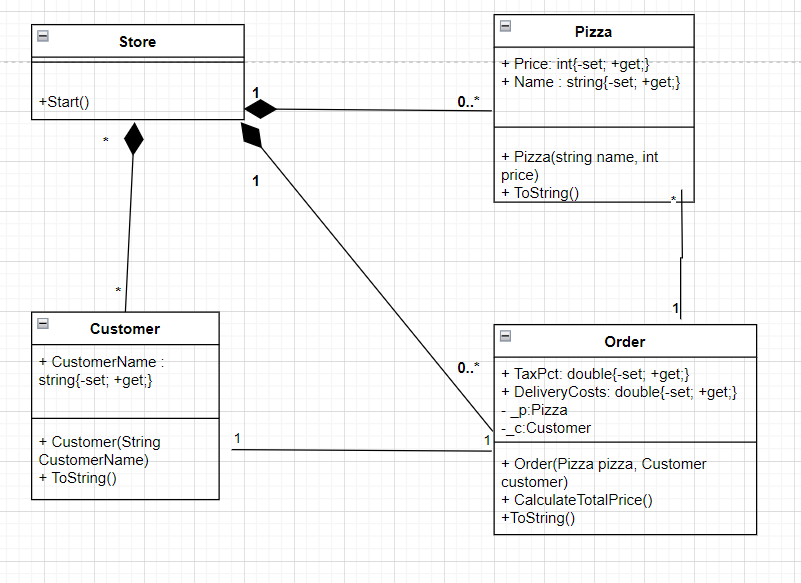
\includegraphics[scale=1]{img/UML1ClassDia.PNG}
    \caption{}
\end{figure}



\newpage
\section{Sequence Diagram}

\begin{figure}[htbp]
    \center
    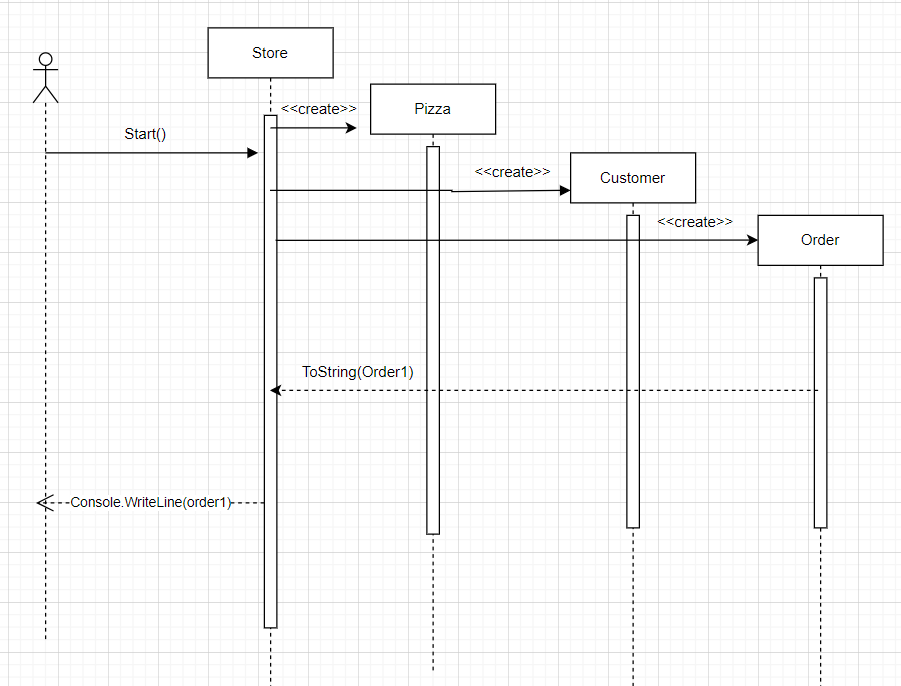
\includegraphics[scale=0.8]{img/UML1Sekvensdia.PNG}
    \caption{Viser kun dannelsen af en order.Hvor i min kode oprettes 3 pizza objekter, 3 customer objekter og 3 Order objekter, som bliver sendt til store og derefter displayed til aktøren }
\end{figure}


\newpage
\section{Implement Design Class}

\urlstyle{https://www.youtube.com/}

\newpage



% ------------------------------------------------------------------------------
% Reference and Cited Works
% ------------------------------------------------------------------------------

\bibliographystyle{IEEEtran}
\bibliography{References.bib}

% ------------------------------------------------------------------------------

\end{document}
